\documentclass[a4paper, twocolumn]{article}
\usepackage[utf8]{inputenc}
\usepackage[spanish]{babel}
\usepackage[T1]{fontenc}
\usepackage[pdftex, hidelinks,
            pdftitle={LaTeX Paper Template},
            pdfauthor={Erik Sven Vasconcelos Jansson},
            pdfsubject={LaTeX Paper Template},
            pdfkeywords={template}]{hyperref}

\usepackage{bm}
\usepackage{caption}
\usepackage{listings}
\usepackage{pdfpages}
\usepackage{booktabs}
\usepackage{mathtools}
\usepackage{blindtext}
\usepackage{algorithmic}
\usepackage{graphicx}
\usepackage{courier}
\usepackage{acronym}
\usepackage{amssymb}
\usepackage{amsthm}
\usepackage{siunitx}
\usepackage{algorithm}
\usepackage{newpxtext, newpxmath}
\usepackage[capitalize, noabbrev]{cleveref}
\usepackage[activate={true, nocompatibility}, final,
            tracking=true, kerning=true, spacing=true,
            factor=1100, stretch=10, shrink=10]{microtype}

\DeclareCaptionFormat{modifiedlst}{\rule{\linewidth}{0.85pt}\\[-2.9pt]#1#2#3}
\captionsetup[lstlisting]{format =  modifiedlst,
labelfont=bf,singlelinecheck=off,labelsep=space}
\lstset{basicstyle=\footnotesize\ttfamily,
        breakatwhitespace = false,
        breaklines = true,
        keepspaces = true,
        language = C++,
        showspaces = false,
        showstringspaces = false,
        frame = tb,
        numbers = left,
        numbersep = 5pt,
        xleftmargin = 16pt,
        framexleftmargin = 16pt,
        belowskip = \bigskipamount,
        aboveskip = \bigskipamount,
        escapeinside={<@}{@>}}

\graphicspath{{figures/}}
\title{\vspace{-1.5em}\textbf{Efecto Hall en p-Germanium}}
\author{{\textbf{Félix Rodríguez Lagonell}} \\
        {\href{mailto:erija578@student.liu.se}
        {\texttt{<frodrigue1117@alumno.uned.es>}}} \\
        {Técnicas Experimentales IV - UNED}}
\date{Septiembre 2021}
\begin{document}

    \maketitle

    \begin{abstract} Verificamos la ecuación de Eötvös para la variación de la tensión superficial en función de la temperatura del líquido mediante el método del anillo o de Du Nouy. \end{abstract} % \tableofcontents
    \section{Introducción} \label{sec:introduction} \subsection{Efecto Hall}

Se conoce como efecto Hall a la aparición de un campo eléctrico en el interior de un conductor por el que circula una corriente $I$ en presencia de un campo magnético $B$. Las cargas que circulan por el conductor están sometidas a la fuerza de Lorentz

\begin{equation}
	\overrightarrow{F} = q(\overrightarrow{v}x\overrightarrow{B})
\end{equation}

Con lo cual aparece una fuerza magnética en los portadores de carga que los reagrupa a ambos lados del conductor de anchura $d$, apareciendo así una diferencia de pontencial en el conductor que origina un campo eléctrico perpendicular al campo magnético. Este campo eléctrico es el denominado campo Hall $E_H$, y ligada a él aparece la tensión Hall $V_H$ según la fórmula

\begin{equation}
	V_H = R_H\frac{IB}{d}
\end{equation}

Donde la constante $R_H$ se conoce como constante de Hall y equivale a

\begin{equation}
	R_H = \frac{1}{nq}
\end{equation}

Siendo $n$ la densidad de portadores de carga y $q$ la carga correspondiente. Además, según \cite{movilidad}, dicha constante se puede relacionar con la conductividad $\sigma$ y con la movilidad $\mu_H$ mediante la ecuación

\begin{equation}
	\mu = R_H \sigma
\end{equation}

\subsection{Efecto Hall y magnetorresistencia}

La magnetorresistencia, descubierta por William Thomson en 1857, es la propiedad que tienen algunos materiales de variar su resistencia eléctrica cuando son sometidos a un campo magnético. Este fenómeno puede relacionarse con el efecto Hall a través de la Ley de Ohm.

\begin{equation}
	R = \frac{V}{I}
\end{equation}

\subsection{Efecto Hall y temperatura}

Un semiconductor puede clasificarse según su conductividad en intrínseco y extrínseco. En los semiconductores intrínsecos los agentes conductores son los electrones y huecos que el material es capaz de generar térmicamente. El p-Germanium es un semiconductor extrínseco ya que es un semiconductor (intrínseco) dopado con materiales que lo proveen de un exceso de huecos para favorecer la conducción a bajas temperaturas. Partiendo del modelo clásico, la conductividad total será la suma de las contribuciones individuales de cada tipo de portador de carga libre, según la expresión

\begin{equation}
	\sigma = n_p \mu_p + n_h \mu_h
\end{equation}

Siendo $n_{p,h}$ la densidad de portadores y $\mu{p,h}$ la movilidad (el subíndice se refiere a portadores y huecos). Aplicando la estadística de Fermi-Dirac a la anterior ecuación y teniendo en cuenta que ambas poblaciones siguen la ley de acción de masas o del equilibrio $n_p n_h = n_i^{2}$ tenemos que se cumple

\begin{equation}
	\sigma = \sigma_0 e^{\frac{-E_g}{2K_bT}}
\end{equation}

Donde $\sigma_0$ es un prefactor que depende de la movilidad y la densidad de estados efectivos en las bandas de conducción y valencia, $E_g$ representa la energía del intervalo prohibido, $K_b$ es la constante de Boltzmann y $T$ la temperatura.
    \section{Metodología} \label{sec:related_work} Contamos con muestras de cristales de fluoruro de litio (LiF) y bromuro de potasio (KBr) y un dispositivo experimental controlado por ordenador que contiene un tubo de rayos X cuyo ánodo es de cobre. El dispositivo dirige los rayos X hacia las muestras cristalinas. Mediante el programa COBRA registraremos las medidas del espectro de rayos X para dichos cristales en función del ángulo de incidencia de entre aproximadamente 5º y 45º, haciendo cinco etapas para la toma de datos de LiF, en las que comenzamos con una diferencia de potencial de 13kV y luego iremos aumentando de tres en tres kV hasta alcanzar los 25kV. Para el KBr llevaremos a cabo una única medida a 25kV.

Todas aquellas medidas que tengan incertidumbre asociada será explícitamente mencionado. Para aquellas magnitudes indirectas se calculará el error asociado según la fórmula habitual

\begin{equation}
	\Delta{A_i} = |\frac{\partial A}{\partial \alpha_i}|\Delta \alpha_i
\end{equation}

    \section{Implementación} \label{sec:implementation} TEXT
    \section{Resultados} \label{sec:results} En primer lugar calcularemos el caudal que circula por el tubo capilar. Pare ello aplicamos la ecuación (\ref{eq_caudal}) donde el volumen lo calculamos a partir de la densidad del agua $\rho = 10^3 kg/m^3$, de tal forma que tendríamos $Q = \frac{M}{\rho t}$. A partir de los datos de altura, calcularemos también la diferencia de presión $\Delta p$ entre los extremos del capilar, que vendrá dada por $\Delta p = \rho gh$ siendo $g = 9.8 m/s^2$ la aceleración de la gravedad. Con estos datos representamos la relación entre el caudal y la presión en la figura (\ref{figure_caudal}), además del correspondiente ajuste por mínimos cuadrados que corresponden a la región de flujo laminar.

\begin{figure}[t]
	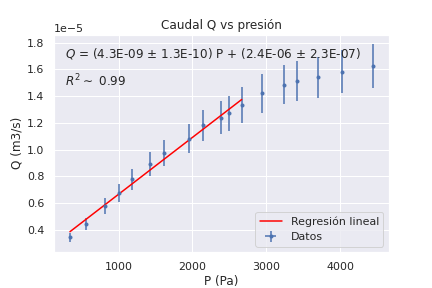
\includegraphics[width=\linewidth]{caudal_vs_presion}
	\caption{Caudal volumétrico de agua en función de $\Delta p$}
	\label{figure_caudal}
\end{figure}

Hay que notar que la recta ajustada no pasa por el origen, sino que predice un caudal nulo para un valor negativo de $\Delta p$, por lo tanto debemos corregir el valor de $\Delta p$ para obtener una recta que efectivamente pase por el origen. En este sentido si identificamos la ecuación de la recta de la figura (\ref{figure_caudal}) tal que $0 = mP+b$ obtenemos un factor de corrección dado por $P' = \frac{b}{m}$. Dado que $\Delta p$ será transformado a $\Delta p'$, debemos tener en cuenta la propagación de errores de dicha transformación, es decir $\epsilon_{p'} = \epsilon_{p} + |\frac{\epsilon_{b}}{m}| + |\frac{b\epsilon_{m}}{m^2}|$. En la figura (\ref{figure_caudal_corregida}) vemos el nuevo ajuste lineal. En este caso comprobamos que se conserva el valor de la pendiente, que el término independiente es prácticamente cero y que los errores en el eje de presión se han incrementado.

\begin{figure}[t]
	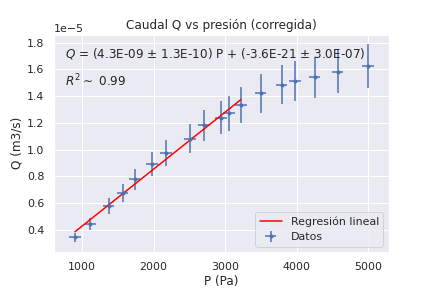
\includegraphics[width=\linewidth]{caudal_vs_presion_corregida}
	\caption{Caudal volumétrico de agua en función de $\Delta p'$ corregida}
	\label{figure_caudal_corregida}
\end{figure}

En términos generales vemos que el caudal es directamente proporcional a la presión en una región que identificamos con el flujo laminar del fluido, dado por el ajuste de mínimos cuadrados, hasta llegar a un punto de aparición de un codo, el cual representa el punto de transición hacia el régimen turbulento. La propagación de errores hace énfasis en este tramo (turbulento) de la dificultad de hallar un valor de caudal lo suficientemente certero.

Mediante la ley de Hagen-Poiseuille, ecuación (\ref{eq_caudal}), identificamos el factor $\frac{\pi r^4 \Delta p}{8\mu L}$ con la pendiente de la regresión lineal, de tal manera que $\mu = \frac{\pi r^4 \Delta p}{8\alpha L}$ donde $\alpha = (4.3 \pm 0.13)\cdot 10^{-9}m^3/Pa\cdot s$. Así pues obtenemos que la viscosidad dinámica es $\mu = (3.2 \pm 0.4) \cdot 10^{-3} Pa \cdot s$, valor que difiere notablemente de su análogo teórico $\mu_t = 0.001 Pa \cdot s$ a una temperatura de 20ºC, siendo el valor experimental tres veces mayor mayor que el valor teórico. Estas diferencias pueden deberse a una discordancia de temperaturas a la que se ha calculado la viscosidad, pues en nuestro caso el laboratorio se encontraba a 27ºC. Además, debido a la propia disposición del dispositivo experimental, no podemos garantizar la exactitud de los valores medidos (distancia, presión, tiempo), que sin un análisis de errores experimentales influye negativamente en los cálculos sucesivos. Por otro lado, la densidad del agua (ideal) para nuestros cálculos no corresponde no el agua utilizada en nuestro experimento.

A partir de estos datos experimentales y gracias a la ecuación (\ref{eq_reynolds}) podemos calcular el número de Reynolds (recordar que $U = \frac{Q}{\pi r^2}$). Los datos correspondientes los podemos ver en la tabla (\ref{table_exp}). Los datos inferiores a la línea horizontal central representan aquellos que corresponden al régimen laminar y con los que se llevó a cabo la regresión lineal (Q vs $\Delta p'$). 

Examinando los datos podemos confirmar el comportamiento $\Delta p \propto Q \propto U$, pues al aumentar la presión aumentará el caudal y, por consiguiente, la velocidad media del agua dentro del tubo capilar. Además comprobamos el régimen laminar para todos aquellos valores que, sumando su correspondiente incertidumbre, están dentro del límite $Re < 2000$. Sin embargo, aunque no obtenemos ningún valor para el número de Reynolds que esté por encima de dicho límite, sí reconocemos la transición al régimen turbulento para todos aquellos valores que sumando la incertidumbre están en el rango $2000<Re<3000$. Como hemos visto, obtenemos, en general, valores inferiores a los esperados con incertidumbres muy altas (sobretodo en régimen transitorio).

También podemos ver en la tabla (\ref{table_exp}) los valores calculados para el coeficiente de resistencia $\lambda$ según la ecuación (\ref{eq_lambda}) y (\ref{eq_lambda_reynolds}). Aunque dichos valores tienen una incertidumbre tal que solapan en rango unos con otros, es importante recalcar que tienen una incertidumbre muy alta (pues son función del número de Reynolds), tanto que el error relativo para este coeficiente está en el rango de entre 30\% y el 40\%, cumpliéndose el 30\% para todos los valores de $\lambda_{64}$. 

En la figura (\ref{figure_lambda}) hemos representado los datos para $\lambda$ en función de $Re$. Las líneas representan las soluciones a la ecuación (\ref{eq_karmann_prandtl}) característica del régimen turbulento. Se ha preferido graficar dichas líneas para el régimen laminar (donde no son válidas) para observar su comportamiento. Podemos identificar entonces que la solución de la ecuación trascendente que más se asemeja a nuestros datos es la línea (morada) que está justo por encima de nuestros puntos experimentales para los valores más altos del número de Reynolds.

Podemos hacer énfasis en el régimen turbulento mediante una presentación logarítmica de nuestros datos. En la figura (\ref{figure_lambda_log}) podemos ver el comportamiento lineal de $log (\lambda)$ frente a $log (Re)$ para el régimen laminar y su correspondiente punto de inflexión hacia el régimen turbulento, marcado por un cambio de tendencia con pendiente positiva.

\begin{figure}[t]
	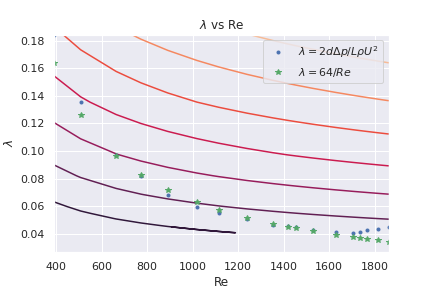
\includegraphics[width=\linewidth]{3lambda_nolog_noerror}
	\caption{Diagrama de Moody. Comportamiento del coeficiente de resistencia $\lambda$ según el número de Reynolds. Las líneas representan las soluciones a la ecuación (\ref{eq_karmann_prandtl}) de Karmann-Prandtl. No se incluyen barras de error debido a su gran tamaño.}
	\label{figure_lambda}
\end{figure}

\begin{figure}[t]
	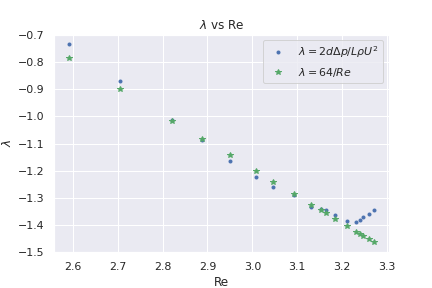
\includegraphics[width=\linewidth]{2lambda_log_noerror}
	\caption{Diagrama de Moody logarítmico para el coeficiente de resistencia. No se incluyen barras de error debido a su gran tamaño.}
	\label{figure_lambda_log}
\end{figure}
    \section{Conclusiones} \label{sec:conclusions} En esta práctica se ha estudiado la estuctura cristalina del LiF y el KBr mediante la difracción de rayos X generados por un ánodo de cobre. Mediante la aplicación directa de la Ley de Bragg hemos calculado los valores de distancia interplanar y parámetro de red, obteniendo valores muy cercanos a sus correspondientes teóricos.

Gracias a la Ley de Bragg y el entendimiento de la radiación de frenado (o bremsstrahlung) hemos podido calcular experimentalmente el valor de la constante de Planck $h = (5.5 \pm 0.9)\cdot 10^{-34} J \cdot s$. Aunque dicho valor experimental difiere notablemente del valor teórico $h = 6.626 \cdot 10^{-34} J \cdot s$, siendo el error relativo entorno a un 17\%, tenemos que el rango de incertidumbre es lo suficientemente alto como para englobar el valor real. Esta diferencia radica principalmente en el error que supone la selección visual de los ángulos mínimos de radiación de frenado.

    \nocite{*} % TODO: remove
    \bibliographystyle{abbrv}
    \bibliography{paper}
    \appendix

    \section{Tablas}

\begin{table}[h]
	\centering
%	\begin{adjustwidth}{-2cm}{}
		\begin{tabular}{cccc}
			\toprule
			%\multicolumn{1}{c}{} & \multicolumn{3}{c}{Distancia (cm)} \\
			%\cmidrule(r){2-4}
$F (N) \cdot 10^{-3}$   &   $T (K)$   &   $\sigma (Nm^{-1}) \cdot 10^{-3}$   &   $\sigma V_{m}^{2/3} (Jmol^{-2/3}) \cdot 10^{-6}$ \\
\midrule
$5.4 \pm 0.1$   &   $352 \pm 1$   &   $44.1 \pm 0.8$   &   $30.3 \pm 0.6$  \\
$5.6 \pm 0.1$   &   $344 \pm 1$   &   $45.7 \pm 0.8$   &   $31.4 \pm 0.6$  \\
$6.0 \pm 0.1$   &   $339 \pm 1$   &   $49.0 \pm 0.8$   &   $33.6 \pm 0.6$  \\
$6.2 \pm 0.1$   &   $334 \pm 1$   &   $50.6 \pm 0.8$   &   $34.8 \pm 0.6$  \\
$6.4 \pm 0.1$   &   $328 \pm 1$   &   $52.2 \pm 0.8$   &   $35.9 \pm 0.6$  \\
$6.9 \pm 0.1$   &   $322 \pm 1$   &   $56.3 \pm 0.8$   &   $38.7 \pm 0.6$  \\
$7.1 \pm 0.1$   &   $316 \pm 1$   &   $57.9 \pm 0.8$   &   $39.8 \pm 0.6$  \\
$6.9 \pm 0.1$   &   $309 \pm 1$   &   $56.3 \pm 0.8$   &   $38.7 \pm 0.6$  \\
$7.2 \pm 0.1$   &   $303 \pm 1$   &   $58.8 \pm 0.8$   &   $40.4 \pm 0.6$  \\
$8.2 \pm 0.1$   &   $299 \pm 1$   &   $66.9 \pm 0.8$   &   $46.0 \pm 0.6$  \\
$8.2 \pm 0.1$   &   $297 \pm 1$   &   $66.9 \pm 0.8$   &   $46.0 \pm 0.6$  \\
$8.5 \pm 0.1$   &   $295 \pm 1$   &   $69.4 \pm 0.8$   &   $47.6 \pm 0.6$  \\
			\bottomrule
		\end{tabular}
		\caption{Resultados experimentales. Todos los resultados se han llevado a cabo con el mayor número de decimales posibles marcados por la precisión del ordenador.}
		\label{table_exp}
%	\end{adjustwidth}
\end{table}

\section{Tratamiento de incertidumbres}

\begin{itemize}
	
	\item \textbf{Tensión superficial}
	\[\mathrm{\Delta \sigma = \left\vert \frac{1}{4\pi r} \Delta F\right\vert }\]
	
	\item\textbf{Eötvös}
	\[\mathrm{\Delta \left( \sigma V^{2/3} \right) = \left\vert V^{2/3} \Delta \sigma \right\vert}\]
	
	\item\textbf{Temperatura crítica}
	\[\mathrm{\Delta T_{k} = \left\vert \frac{1}{k} \Delta b\right\vert  + \left\vert \frac{-b}{k^{2}} \Delta k\right\vert}\]
	
\end{itemize}

\end{document}
